\chapter{Methods and Procedure}
\label{chapter:methods}

In figure \ref{fig:image}, the processing pipeline for this project is shown.

\begin{figure}[h!]
    \centering
    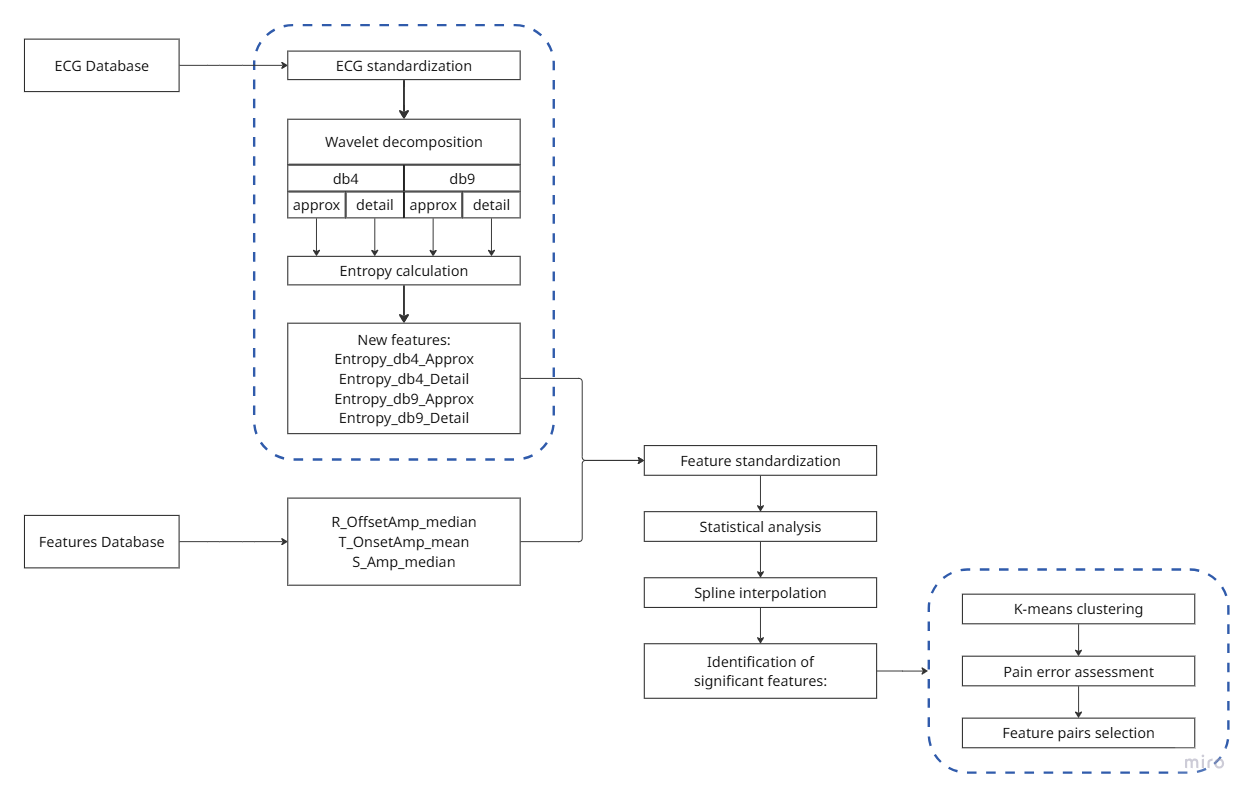
\includegraphics[width=1.0\textwidth]{image.png}
    \caption{Processing pipeline.}
    \label{fig:image}
\end{figure}

\section{Database Acquisition}
In this project, two databases were used: one has data from an \ac{ecg} signal while the other contains features extracted from that \ac{ecg}, as described in the article by Bruna et al \cite{Alves2024}.

The protocol that was carried out to create the databases began with a 5-minute baseline period, during which only physiological signals were collected while participants sat in a relaxed position without any stimuli. 
Next, participants viewed a 10-minute video composed of segments from comedy, horror or documentary films to elicit positive, negative or neutral emotional states, respectively. 
After the video, another 5-minute stimuli-free period was conducted. 
Following this, participants immersed their non-dominant hand in a tank of cold water (7 ± 1°C), inducing pain through a Cold Pressor Test(\ac{cpt}), and reported their pain using the \ac{nps} at four key points: before immersing their hand, when pain was first felt (Pain Threshold), when the pain became unbearable (Pain Tolerance) and 3 minutes after removing their hand from the water. 
The CPT section ended when the limit of pain tolerance was reached, or after 2 minutes if the participant didn’t reach theirs before that. 
Finally, the 5-minute period with no stimuli was repeated, being characterized as a rest period. 
This process is depicted in figure \ref{fig:database}. 

\begin{figure}[h!]
    \centering
    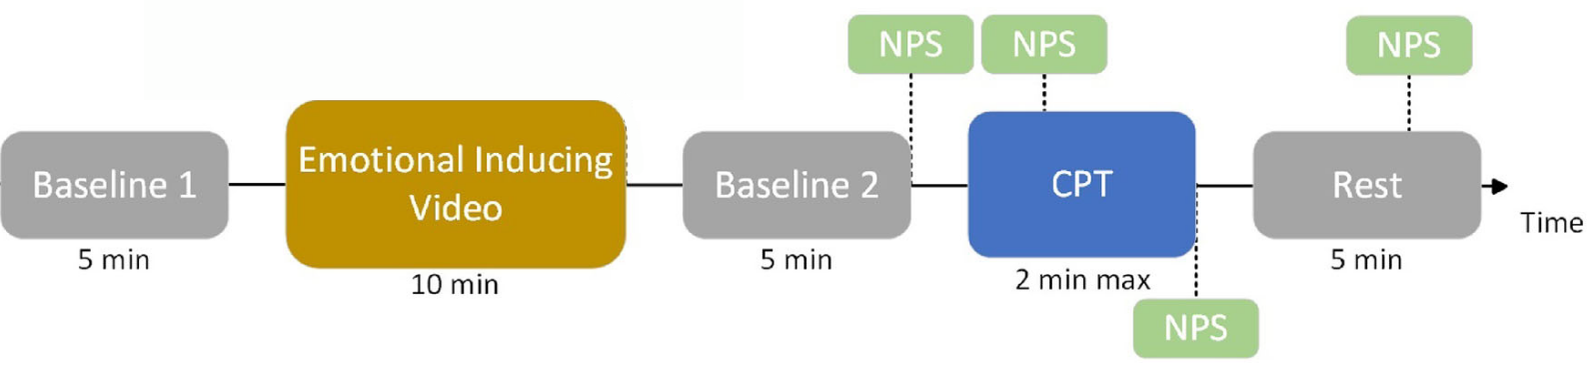
\includegraphics[width=1.0\textwidth]{database.png}
    \caption{Scheme of the protocol applied to obtain the database. (Adapted from \cite{Alves2024})}
    \label{fig:database}
\end{figure}

During the study, three physiological signals were recorded, more precisely, ECG, EDA and EMG from trapezius and triceps muscles. The ECG was recorded in a database, that was later used in this project.
Following up in the article, heart rate (HR), the amplitude of wave peaks, the amplitude of onsets and offsets of the waves, the distance between consecutive onsets and offsets and the distance between consecutive peaks were extracted in the form of time series, using 10-second windows with 50\% overlap. 
Then, for all of these, statistical metrics, like the mean, median and variance, were computed for each window, resulting in 237 features that were later processed. 
These are all included in the features database, also used in this project.



\section{Feature Extraction}
In the aforementioned article, the features of the ECG that can be used to best describe pain are defined.
Hence, the top four features were selected for analysis, namely, the median of the R wave offset amplitude, the median of the T wave onset amplitude, and the mean and median of the S wave peak amplitude.

To enhance this research, new features were sought out. 
For this reason, analysis of the ECG database itself was deemed necessary. 


\subsection{ECG Data Exploration}
When looking at the time series of the signal, in figure \ref{fig:ecg}, it's noticeable that the range of amplitudes of the QRS complex is way bigger than that of the P and T waves.
To tackle this, the ECG signal was standardized according to equation \ref{eq:1}, where X is the original ECG, $\mu$ is the mean, $\sigma$ is the standard deviation and Z is the standardized signal, which has mean zero and standard deviation one. 
This means the range of values is the same for all participants, which allows for comparison between them.

\begin{equation} \label{eq:1}
Z = \frac{X-\mu}{\sigma}
\end{equation}

% \begin{figure}[h!]
%     \centering
%     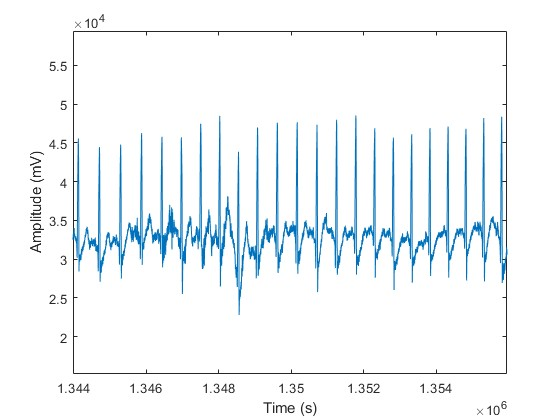
\includegraphics[width=0.9\textwidth]{ecg.jpg}
%     \caption{Section of the ECG signal of a participant.}
%     \label{fig:ecg}
% \end{figure}

\begin{figure}[htbp]
    \centering
    \begin{minipage}{0.45\textwidth}
        \centering
        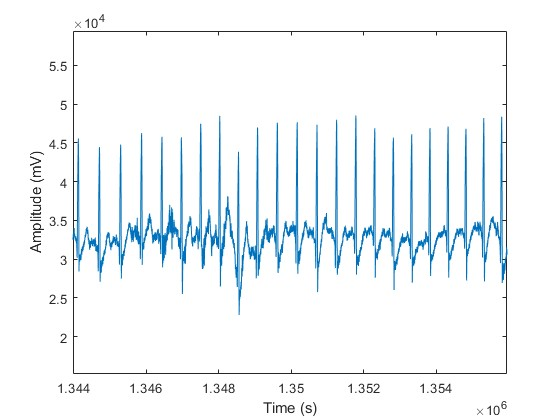
\includegraphics[width=6.5cm]{ecg}
        \caption{Section of the ECG signal of a participant.}
        \label{fig:ecg}
    \end{minipage}
    \hfill
    \begin{minipage}{0.45\textwidth}
        \centering
        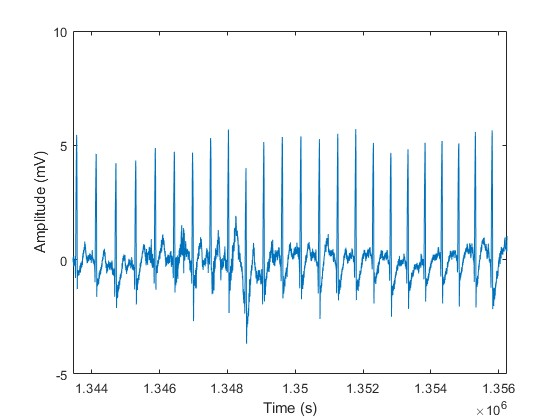
\includegraphics[width=6.5cm]{normalized ecg}
        \caption{Section of the standardized ECG signal of a participant.}
        \label{fig:normalized_ecg}
    \end{minipage}
\end{figure}

Once the signal was standardized, fluctuations were noticed in the time series.
By removing high frequencies from the signal, by filtering for example, these would be alleviated.
However, there could be information related to pain associated to those frequencies.
%The solution to solve both of these problems was to decompose the signal in wavelets. 

(Falar das famílias de wavelets para análise de ECGs)

To choose the best type of wavelet, two criteria were established: one's format should be similar to that of the ECG wave and the other should have a higher frequency, while still maintaining its smoothness.
Accordingly, Daubechies-4 ('db4') and Daubechies-9 ('db9') were chosen.
Regarding the number of levels of decomposition, as can be seen in figure \ref{fig:wavelets2}, when there are two levels the R peak is noticeable in the detail, which is not something we want to highlight.
Therefore, only one level of decomposition was applied.

\begin{figure}[h!]
    \centering
    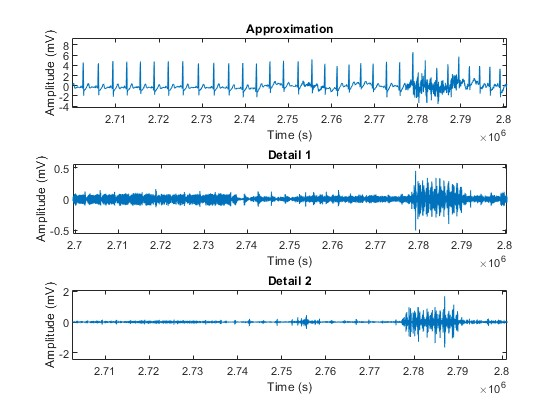
\includegraphics[width=1.0\textwidth]{wavelets 2.jpg}
    \caption{Daubechies-4 Wavelet Decomposition - level 1.}
    \label{fig:wavelets2}
\end{figure}


\subsection{Entropy Calculation}
Since the features associated with the ECG waves had already been extracted and analysed, it was decided that the entropy of the decomposed signal would be calculated.
Using the same window as the other features, that is, 10 seconds with 50\% superposition, 



\section{Data Analysis}
To do the optimal processing of the features, five participants were selected at random, while ensuring the videos watched by them were different. 
Once this was done, graphics of the features in function of time were plotted for each participant. 
An example can be seen in figure 3, in which a clear change can be seen when the participant dips their hand in water, feeling pain. 

Once the features were standardized, a statistical analysis was done using histograms of the features of the five participants, depicted in figure 7. 
These show that the features don’t have a normal distribution, so it makes sense to use the median and interquartile range as the central tendency and dispersion measures, respectively. 
These, calculated for each feature, were considered “new features”, which will be analysed further.

The goal of this project is to select features that distinguish pain from no pain. 
To do this, it’s important that each step of the protocol has the same size, so that they’re comparable. 
With this aim, linear interpolation was done in each step, so they all had exactly the equivalent to 60 seconds of length, or 60 values, to be precise. 
The result of this method is portrayed in figure 8.









